
\chapter{Causality}

\index{causal relationship}
\index{observational study}
\index{controlled experiment}

I must now ask you to reach in your memory banks alllll the way back to
Chapter~10 of the \textit{previous} volume of this book series. That chapter,
entitled ``Interpreting Data,'' dealt with association vs.~causality,
confounding factors, controlled experiments vs.~observational studies, and
related topics. The key question we addressed was how to interpret a
statistical association between variables. If two variables are correlated,
then they're correlated...but how confident can we be that there's a
\textbf{causal} relationship between them -- which is what we usually care
about?

\index{causal diagram}
\index{barbecue}
\index{cancer}

\vspace{-.1in}
\begin{figure}[ht]
\begin{minipage}{6in}
\raisebox{-.5\height}{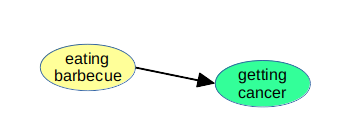
\includegraphics[width=0.45\textwidth]{causalDiagram.png}}
\raisebox{-.5\height}{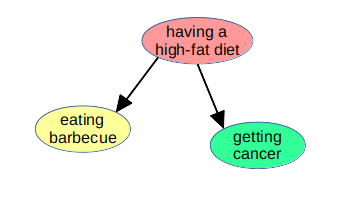
\includegraphics[width=0.45\textwidth]{causalDiagram2.png}}
\vspace{-.15in}
\caption{Causal diagrams, each expressing a hypotheses about the causality
among variables.}
\label{fig:causalDiagrams}
\end{minipage}
\end{figure}
\vspace{-.05in}

The tool we used for this analysis was the \textbf{causal diagram}, examples of
which appear in Figure~\ref{fig:causalDiagrams}. Each bubble represents one
variable. Arrows pointing from one bubble to another asserts a causal
relationship between the two: that the value of one is not merely
\textit{associated with}, but is partially \textit{responsible for}, the value
of the one pointed at. 

If you remember that particular example, there was an observational study
suggesting that eating barbecue can increase one's risk of various types
cancer. Assuming that an association between the two variables was in fact
discovered, the two sides of Figure~\ref{fig:causalDiagrams} represent
competing theories as to the reasons for that association.

The question we'll ask in this chapter is as follows: given a data set, is
there any way to actually \textit{tell} which of several competing causal
theories is true? In other words, if we have more than one hypothesis giving
alternate explanations for how the patterns in the data set arrived, can the
\textit{data itself} be used to judge between them?

And the answer is: sometimes. Let's learn when it can, and when it cannot.

\section{The bad news: identical ``skeletons''}

Before I get you too excited, let me say right at the outset that there are
times when the data fails us in our quest to nail this down. This happens when
the \textbf{skeleton}s of the two causal models are identical.

\index{skeleton (of a causal diagram)}
\index{smoking}
\index{depression}

The skeleton of a causal diagram is simply the diagram you get if you
\textit{remove the arrowheads}. Consider the two competing models in
Figure~\ref{smokingDepression}. An observational study some years ago found an
association between smoking cigarettes and experiencing clinical depression,
and made the claim that therefore one of the many detriments to smoking
(besides heart disease, lung cancer, and other things) was an emotional one.
That represents the causal model on the left side of the diagram. But some
objected and said, ``wait a minute...couldn't it instead be the case that
people who are going through depression are seeking ways to cope with it, and
that substances like nicotine could be one of those ways?'' This
depression-causes-smoking hypothesis is on the right side. 

\vspace{-.15in}
\begin{figure}[ht]
\begin{minipage}{6in}
\raisebox{-.5\height}{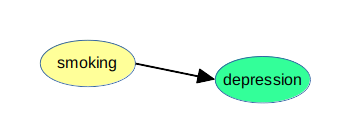
\includegraphics[width=0.45\textwidth]{smokingDepression.png}}
\raisebox{-.5\height}{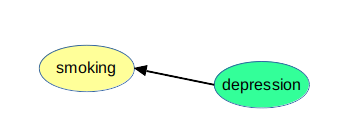
\includegraphics[width=0.45\textwidth]{depressionSmoking.png}}
\vspace{-.15in}
\caption{Does smoking cause depression...or does depression lead to smoking?}
\label{smokingDepression}
\end{minipage}
\end{figure}
\vspace{-.05in}

Unfortunately there is no way to resolve this by looking at the data alone.
This is because if you remove the (one) arrowhead, you get the same skeleton
(Figure~\ref{smokingDepressionSkeleton}). Note that ``the same skeleton'' means
merely \textit{the same bubbles are connected to the same bubbles.} It does
\textit{not} have anything to do with where those bubbles are positioned on the
page.

\vspace{-.1in}
\begin{figure}[ht]
\begin{center}
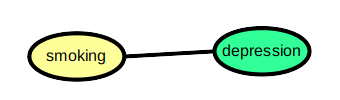
\includegraphics[width=0.8\textwidth]{smokingDepressionSkeleton.png}
\vspace{-.15in}
\caption{The bad case: both causal diagrams have the \textit{same} skeleton.}
\label{smokingDepressionSkeleton}
\end{center}
\end{figure}
\vspace{-.05in}

In this case, the only way to resolve which of the causal models is the true
one is to investigate the phenomenon on the ground. We have to study the
mechanisms -- physical and societal -- by means of which each of them might
plausibly cause the other. Medical researchers could explore the effects of
nicotine on the human brain, and determine whether there is a mechanism by
which serotonin is reduced. Social psychologists could conduct surveys and
focus groups and learn how often cigarettes are sought by victims of depression
and why. But the data itself will not give a verdict.


\section{The good news: different ``skeletons''}

Often, though, the situation isn't that dire. Consider the controversy raised
in one of my recent freshman seminars. The class was discussing the invention
of chopsticks, and the impact that may have had on eastern culture as well as
culinary techniques. One student made a different kind of claim. He said,
``this is why so many of the great video game players in the world are from
Asian countries! When kids from those regions grow up using chopsticks, it
demands more attention to fine motor skills than using a fork would. And when
they develop this terrific finger-eye coordination at a young age, it leads to
greater expertise with a controller or keyboard. Thus they are better equipped
to compete in high-level gaming.''

Perhaps. But as I listened to this student, I couldn't help remembering what my
own boys told me: that many of the Asian countries place a higher cultural
value on video games than we do in the western world. Apparently,
high-achieving video game players are afforded the same fame and fortune in
South Korea or Japan that our NFL and NBA players are in the U.S. They are
awarded lucrative contracts, perform paid testimonial advertising, give
autographs to cheering throngs, and so forth. It stands to reason, then, that a
culture which rewards excellent video game play would produce excellent video
gamers \textit{regardless} of whether those players used forks or chopsticks.

\vspace{-.15in}
\begin{figure}[ht]
\begin{center}
\raisebox{-.5\height}{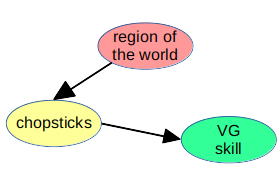
\includegraphics[width=0.4\textwidth]{chopsticksVG.png}}
\quad
\raisebox{-.5\height}{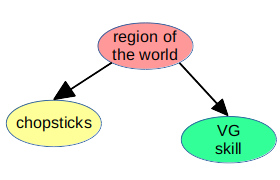
\includegraphics[width=0.4\textwidth]{regionVG.png}}
\vspace{-.05in}
\caption{Two competing causal models about why many great video game
players are from Asian countries.}
\label{chopsticksVG}
\end{center}
\end{figure}
\vspace{-.05in}

These two competing hypotheses are illustrated in Figure~\ref{chopsticksVG}.
On the left is my student's model: the region of the world you're in (Asian or
non-Asian) influences whether or not you primarily use chopsticks at your
meals. With this much, I agree. But he then further claims that the use of
chopsticks \textit{causally influences} how good a video game player you are.

The right side of the diagram shows my own mental model: the region of the
world you're in causally influences both chopstick usage \textit{and} video
game prowess. In my model, \textsf{chopsticks} and \textsf{VG skill} are
\textit{associated}, but not \textit{causally} associated.

Now before we go on, consider the following exercise. Without even knowing the
technical detail that comes next, can you figure out how to confirm or refute
my student's (left-hand) causal model? What could you do with the data?

\index{conditional probability}
\index{conditioning@``conditioning on'' (probability)}
\index{confounding factor}

The solution is intuitive to many, but not to all. Simply put, you
\textbf{condition on} the \text{region of the world} variable. This means you
split the data into two groups: those from Asian countries and those from
non-Asians countries. Think about it: if you \textit{considered only Asians},
and discovered that chopstick-using Asians are better video gamers than
non-chopstick-using Asians, then that would lend credence to the hypothesis
that one causes the other. (And the same goes for considering only non-Asians.)
But if you looked only at Asians (or only at non-Asians) and found that
chopsticks and video game skill are \textit{un}correlated, then that pretty
much refutes the hypothesis. Everything in the coming sections is an
elaboration of that principle.

\subsection{Comparing the skeletons}

\index{skeleton (of a causal diagram)}
The reason this example turns out to be one of the ``good news`` cases is that
the skeletons of the causal diagrams are different. Check out
Figure~\ref{chopsticksVGskeleton}. At first glance, you might assume that they
are the same, just as in the smoking/depression example. After all, they're
both chains-of-three nodes. But they're \textit{not} the same. In one,
\textsf{chopsticks} is the bubble with connections to the other two, and in the
other it's \textsf{region of the world}. Just because they're the same shape
doesn't mean they're the same skeleton: the same bubbles have to be connected
to the same bubbles.

\vspace{-.15in}
\begin{figure}[ht]
\begin{center}
\raisebox{-.5\height}{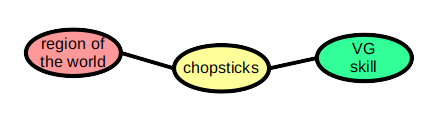
\includegraphics[width=0.45\textwidth]{chopsticksVGskeleton.png}}
\quad
\raisebox{-.5\height}{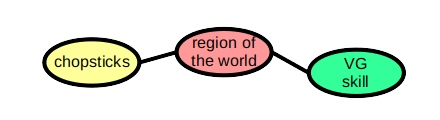
\includegraphics[width=0.45\textwidth]{regionVGskeleton.png}}
\vspace{-.05in}
\caption{The good case: the causal diagrams have \textit{different}
skeletons.}
\label{chopsticksVGskeleton}
\end{center}
\end{figure}
\vspace{-.05in}

And since the skeletons are different, the data can distinguish between the
two, and tell us which causal model (or neither) is likely to be correct.

\subsection{Reasoning about independence}

\index{independence (probability)}

The reason we can use the data to render a verdict on our competing causal
diagrams is that they embody different \textit{independence assumptions}.

Look carefully at the left side of Figure~\ref{chopsticksVG} on
p.~\pageref{chopsticksVG}. If that causal model were true, then
\textsf{chopsticks} and \textsf{VG skill} would not be absolutely independent.
Nor would \textsf{region of the world} and \textsf{VG skill}: after all, if
you're from an Asian country, you're more likely to use chopsticks, and if you
use chopsticks, you're more likely to be good at video games, so of course
the \textsf{region of the world} and \textsf{VG skill} variables are
correlated.

\index{conditional independence}
\index{conditional probability}

However, in that left-hand diagram, \textsf{region of the world} and \textsf{VG
skill} will be \textit{\underline{conditionally} independent given
\textsf{chopsticks}}. In symbols:

\vspace{-.1in}
\begin{samepage}
\begin{align*}
P(\textrm{VG}\ |\ \textrm{region}) \neq P(\textrm{VG})
\end{align*}
\begin{center}
\textit{but}
\end{center}
\vspace{-.1in}
\begin{align*}
P(\textrm{VG}\ |\ \textrm{region},\ \textrm{chopsticks}) =
P(\textrm{VG}\ |\ \textrm{chopsticks})
\end{align*}
\end{samepage}

Why is this? Because in the left-hand diagram, the only reason that knowing
a person's \textsf{region} was of any use to predicting their \textsf{VG skill}
was because it influenced how likely it was that they used \textsf{chopsticks}.
If you actually \textit{have} the information about \textsf{chopsticks}
directly, well then you can toss \textsf{region} out the window. It's
irrelevant at that point.

The right-hand side of Figure~\ref{chopsticksVG} is much different. Its
independence assumptions are that \textsf{VG skill} and
\textit{\textsf{chopsticks}} are conditionally independent given
\textit{\textsf{region}}. Namely:

\vspace{-.1in}
\begin{samepage}
\begin{align*}
P(\textrm{VG}\ |\ \textrm{region}) \neq P(\textrm{VG}) \quad \textrm{(again)}
\end{align*}
\begin{center}
\textit{but}
\end{center}
\vspace{-.1in}
\begin{align*}
P(\textrm{VG}\ |\ \textrm{chopsticks},\ \textrm{region}) =
P(\textrm{VG}\ |\ \textrm{region})
\end{align*}
\end{samepage}
\vspace{-.1in}

This is the flip side of the former case: now, although \textsf{chopsticks} can
tell you something useful about \textsf{VG skill} in a pinch, the primary
influencer of gaming skill is not \textsf{chopsticks}, but
\textit{\textsf{region}}. Once you tell me what region of the world somebody is
from, I have much better information about their possible video game use, and
knowing whether they use chopsticks is no longer of interest to me.

\bigskip

To sum up: both models agree that

\vspace{-.1in}
\begin{align*}
P(\textrm{VG}\ |\ \textrm{region}) \neq P(\textrm{VG}).
\end{align*}
\vspace{-.1in}

But the left one (my student's hypothesis) asserts:

\vspace{-.1in}
\begin{align*}
P(\textrm{VG}\ |\ \textrm{region},\ \textrm{chopsticks}) &=
P(\textrm{VG}\ |\ \textrm{chopsticks})\\
P(\textrm{VG}\ |\ \textrm{chopsticks},\ \textrm{region}) &\neq
P(\textrm{VG}\ |\ \textrm{region}),
\end{align*}
\vspace{-.1in}

while the right one (my own hypothesis) asserts:

\vspace{-.1in}
\begin{align*}
P(\textrm{VG}\ |\ \textrm{region},\ \textrm{chopsticks}) &\neq
P(\textrm{VG}\ |\ \textrm{chopsticks})\\
P(\textrm{VG}\ |\ \textrm{chopsticks},\ \textrm{region}) &=
P(\textrm{VG}\ |\ \textrm{region}).
\end{align*}

(Note carefully the ``='' vs.~``$\neq$'' signs in those equations, because
they're the only difference!)

Armed with this insight, we realize that judging between our alternate causal
models boils down to analyzing the data to see which conditional independence
assumptions actually hold. Let's see how to do that.

\section{Testing the data for conditional independence}

